
\section{Results}
\label{sec:results}

% Note that TeX has a mind of its own when it comes to placing images
% in documents - where a figure appears in the PDF document will often
% be quite different from where it appears in the source code. This is
% a feature, not a bug - it enables LaTeX to produce layouts that
% "flow" better. It only takes a few lines to insert a figure into
% your write-up - I recommend using PNG, JPG or PDF images
% (incidentally, programs like Excel and Matlab will allow you to save
% any plots or figures you generate in those formats). The \figure{}
% command is used to create a new figure.
\begin{figure}[htb]

  \centering  % centers the image in the column

  % replace the second argument below with your filename. I like to
  % place all my figures in a sub-directory to keep things organized
  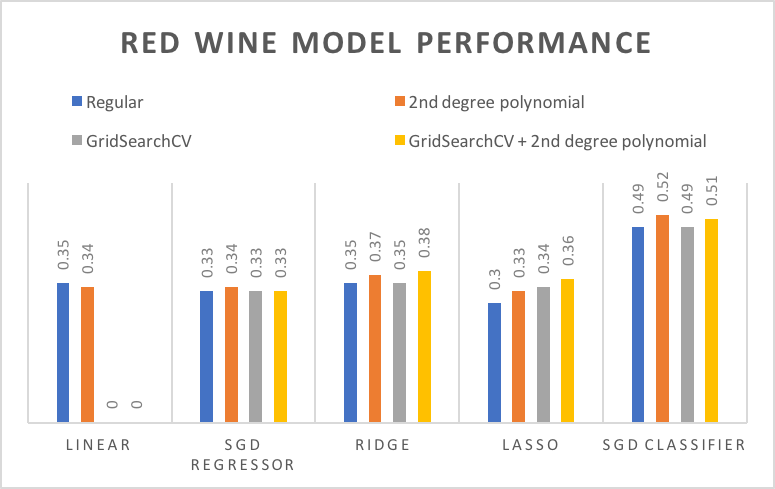
\includegraphics[width=0.47\textwidth]{redwine_score.png}

  % *Every* figure should have a descriptive caption.
  \caption{Graph of red wine model performance at various experimental stages.}

  % The label is a handle you create so that you can refer to this
  % figure (using the \ref{} command) from other parts of your
  % document. LaTeX automatically renumbers figures and updates
  % references when you recompile, so you should do it this way rather
  % than hard-coding in references. Notice that I've also been
  % creating labels for the various sections in the document; I could
  % use \ref{} command to refer to those sections using their labels
  % too.
  \label{fig:tex}

  \end{figure}

  \begin{figure}[htb]

  \centering  % centers the image in the column

  % replace the second argument below with your filename. I like to
  % place all my figures in a sub-directory to keep things organized
  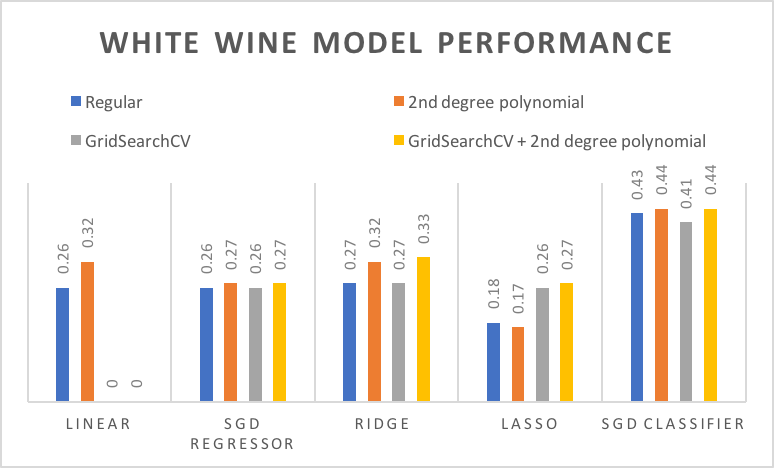
\includegraphics[width=0.47\textwidth]{whitewine_score.png}

  % *Every* figure should have a descriptive caption.
  \caption{Graph of white wine model performance at various experimental stages.}

  % The label is a handle you create so that you can refer to this
  % figure (using the \ref{} command) from other parts of your
  % document. LaTeX automatically renumbers figures and updates
  % references when you recompile, so you should do it this way rather
  % than hard-coding in references. Notice that I've also been
  % creating labels for the various sections in the document; I could
  % use \ref{} command to refer to those sections using their labels
  % too.
  \label{fig:tex}

  \end{figure}
 

  

Overall, our results proved to be pretty interesting. Running \texttt{GridSearchCV} improved the performance of all our models. Trying a second degree polynomial using \texttt{PolynomialFeatures} made our performance even better. Our models performed better for red wine than white wine. This may have been because of an inherent disconnect between the features and the target for the white wine dataset. This isn't really what we expected, since we thought the large number of training examples in the white wine dataset would lead to a better model. However, our main take-away message from our experiments is that a combination of running \texttt{GridSearchCV} and using second degree polynomials is necessary for better model performance.